\chapter{Software Dependencies and Environment}
\label{ch:dependencies}

% ============================================================
\section{Why Dependencies Matter}

A software system is not just the code you write---it is also the code
you \emph{depend on}.  The PQC Secure MAVLink Tunnel relies on
approximately~30 external packages (14~Python, 14~JavaScript/TypeScript,
and a handful of system-level dependencies) that together provide
cryptographic primitives, network protocol parsing, hardware sensor
access, process management, data analysis, and a full web-based dashboard.

Understanding these dependencies is essential for three reasons:

\begin{enumerate}
  \item \textbf{Reproducibility.}  A benchmark result is only meaningful
        if another researcher can recreate the exact software environment.
        A different version of \texttt{liboqs} may produce different
        handshake timings.  A different version of \texttt{pandas} may
        parse CSV files differently.

  \item \textbf{Security.}  Every dependency is an attack surface.
        A vulnerability in \texttt{cryptography} or \texttt{uvicorn}
        could compromise the entire system.  Knowing what you depend on
        is the first step toward auditing it.

  \item \textbf{Maintainability.}  When a dependency releases a breaking
        change, you need to know exactly which parts of your codebase
        are affected.  This chapter provides that map.
\end{enumerate}

\begin{keyinsight}{The Dependency Iceberg}
  The codebase you write is the tip of the iceberg.  Beneath it are
  thousands of lines of library code that do the heavy lifting.
  The \texttt{cryptography} package alone contains over 100{,}000~lines
  of Python and C code.  \texttt{liboqs} contains over 300{,}000~lines
  of C implementing post-quantum algorithms.  Understanding what sits
  beneath your code is not optional---it is a professional responsibility.
\end{keyinsight}

% ============================================================
\section{Dependency Architecture Overview}

The system's dependencies form a layered stack.  At the bottom are
system-level components (the operating system, hardware interfaces,
the C compiler toolchain).  Above those sit the Python and JavaScript
runtimes.  Above those sit the third-party packages.  And at the top
sits the application code.

\begin{center}
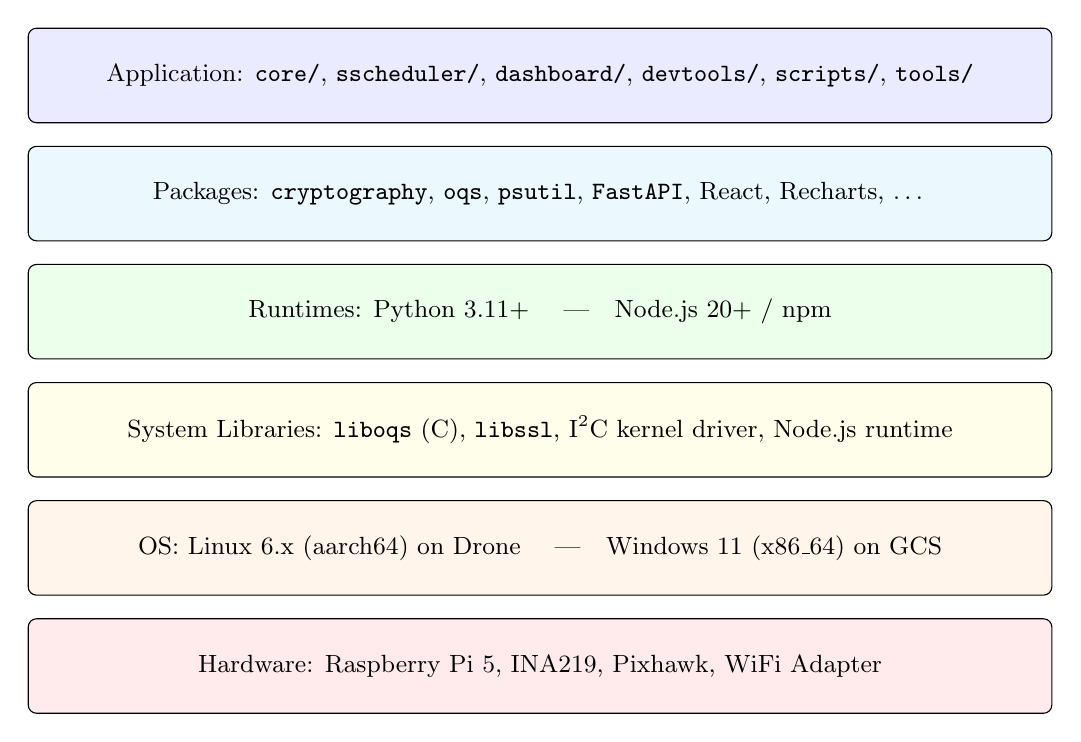
\begin{tikzpicture}[
  layer/.style={draw, rounded corners=3pt, minimum width=13cm, minimum height=1.2cm, font=\small},
]
  \node[layer, fill=red!8]    (hw)  at (0, 0)   {Hardware: Raspberry Pi~5, INA219, Pixhawk, WiFi Adapter};
  \node[layer, fill=orange!8] (os)  at (0, 1.5) {OS: Linux 6.x (aarch64) on Drone \quad|\quad Windows 11 (x86\_64) on GCS};
  \node[layer, fill=yellow!8] (sys) at (0, 3.0) {System Libraries: \texttt{liboqs} (C), \texttt{libssl}, I\textsuperscript{2}C kernel driver, Node.js runtime};
  \node[layer, fill=green!8]  (rt)  at (0, 4.5) {Runtimes: Python 3.11+ \quad|\quad Node.js 20+ / npm};
  \node[layer, fill=cyan!8]   (pkg) at (0, 6.0) {Packages: \texttt{cryptography}, \texttt{oqs}, \texttt{psutil}, \texttt{FastAPI}, React, Recharts, \ldots};
  \node[layer, fill=blue!8]   (app) at (0, 7.5) {Application: \texttt{core/}, \texttt{sscheduler/}, \texttt{dashboard/}, \texttt{devtools/}, \texttt{scripts/}, \texttt{tools/}};
\end{tikzpicture}
\end{center}

Each layer depends on everything below it.  A change at any layer
can ripple upward.  The sections that follow document every component
in the ``Packages'' layer and explain its role in the system.

% ============================================================
\section{Python Backend Dependencies}
\label{sec:deps-python}

The Python backend has two classes of dependencies: those declared
in a \texttt{requirements.txt} file (for the dashboard backend),
and those imported directly by the \texttt{core/} and
\texttt{sscheduler/} packages (installed manually or via conda).

\subsection{The \texttt{cryptography} Package}
\label{sec:dep-cryptography}

\begin{longtable}{p{3.5cm} p{10cm}}
  \toprule
  \textbf{Attribute} & \textbf{Detail} \\
  \midrule
  \textbf{Package name}   & \texttt{cryptography} \\
  \textbf{PyPI URL}        & \url{https://pypi.org/project/cryptography/} \\
  \textbf{Version used}    & $\ge 41.0$ \\
  \textbf{License}         & Apache-2.0 / BSD-3-Clause (dual) \\
  \textbf{Language}         & Python + Rust + C (via OpenSSL) \\
  \textbf{Size}             & $\sim$5\,MB wheel \\
  \bottomrule
\end{longtable}

\paragraph{What it provides.}
The \texttt{cryptography} package is the backbone of all
\emph{classical} cryptographic operations in the system.  It provides:

\begin{itemize}
  \item \textbf{AES-256-GCM} authenticated encryption
        (\texttt{cryptography.hazmat.primitives.ciphers.aead.AESGCM})
  \item \textbf{ChaCha20-Poly1305} authenticated encryption
        (\texttt{cryptography.hazmat.primitives.ciphers.aead.ChaCha20Poly1305})
  \item \textbf{HKDF-SHA256} key derivation
        (\texttt{cryptography.hazmat.primitives.kdf.hkdf.HKDF})
  \item \textbf{HMAC-SHA256} message authentication
        (\texttt{cryptography.hazmat.primitives.hmac.HMAC})
  \item \textbf{SHA-256} hashing
        (\texttt{cryptography.hazmat.primitives.hashes.SHA256})
\end{itemize}

\paragraph{Where it is used.}
\begin{itemize}
  \item \filename{core/aead.py} --- Creates \classname{AESGCM} and
        \classname{ChaCha20Poly1305} cipher objects for the data-plane
        encryption/decryption path.
  \item \filename{core/handshake.py} --- Uses HKDF to derive two
        directional transport keys from the KEM shared secret.
        Uses HMAC for drone PSK authentication.
  \item \filename{core/run.py} --- Passes AEAD algorithm tokens to
        the cipher factory.
\end{itemize}

\begin{designdecision}{Why \texttt{cryptography} and not \texttt{pycryptodome}?}
  The \texttt{cryptography} package delegates to OpenSSL's C
  implementation, benefiting from hardware AES-NI acceleration on
  the GCS (Intel CPU) and NEON-accelerated AES on the Raspberry Pi~5
  (ARM Cortex-A76).  \texttt{pycryptodome} also provides AES-GCM, but
  \texttt{cryptography}'s API is simpler, its maintenance record is
  stronger, and it is the \emph{de facto} standard in the Python
  ecosystem.
\end{designdecision}

\subsection{The \texttt{oqs-python} Package (liboqs)}
\label{sec:dep-oqs}

\begin{longtable}{p{3.5cm} p{10cm}}
  \toprule
  \textbf{Attribute} & \textbf{Detail} \\
  \midrule
  \textbf{Package name}   & \texttt{oqs} (imported as \texttt{oqs}; installed as \texttt{liboqs-python}) \\
  \textbf{GitHub}          & \url{https://github.com/open-quantum-safe/liboqs-python} \\
  \textbf{Underlying C lib}& \texttt{liboqs} 0.10.x \\
  \textbf{License}         & MIT \\
  \textbf{Install method}  & conda (\texttt{oqs-dev} environment) or from source \\
  \textbf{Size}             & $\sim$25\,MB (including compiled C library) \\
  \bottomrule
\end{longtable}

\paragraph{What it provides.}
This is the single most important dependency in the entire system.
\texttt{oqs-python} provides Python bindings to the Open Quantum Safe
\texttt{liboqs} C library, which implements:

\begin{itemize}
  \item \textbf{9~KEM algorithms}: ML-KEM-512, ML-KEM-768, ML-KEM-1024,
        Classic McEliece (348864, 460896, 6688128), HQC-128, HQC-192,
        HQC-256
  \item \textbf{8~Signature algorithms}: ML-DSA-44, ML-DSA-65, ML-DSA-87,
        Falcon-512, Falcon-1024, SPHINCS+-SHA2-128f-simple,
        SPHINCS+-SHA2-192f-simple, SPHINCS+-SHA2-256f-simple
\end{itemize}

\paragraph{Import patterns used.}
The codebase uses two distinct import styles, reflecting different
\texttt{oqs-python} versions:

\begin{lstlisting}[style=python, caption={OQS import patterns in the codebase.}]
# Style 1: Modern flat import
import oqs

kem = oqs.KeyEncapsulation("ML-KEM-768")
sig = oqs.Signature("ML-DSA-65")

# Style 2: Legacy nested import (compatibility)
from oqs.oqs import KeyEncapsulation, Signature

kem = KeyEncapsulation("Kyber768")
\end{lstlisting}

\paragraph{Where it is used.}
\begin{itemize}
  \item \filename{core/handshake.py} --- Creates KEM keypairs
        (\funcname{generate\_keypair}), encapsulates shared secrets
        (\funcname{encap\_secret}), decapsulates
        (\funcname{decap\_secret}), signs challenges
        (\funcname{sign}), and verifies signatures (\funcname{verify}).
  \item \filename{core/suites.py} --- Probes which algorithms are
        available at runtime via \funcname{oqs.get\_enabled\_KEM\_mechanisms()}
        and \funcname{oqs.get\_enabled\_sig\_mechanisms()}.
  \item \filename{sscheduler/benchmark\_policy.py} --- Iterates through
        all available suites.
\end{itemize}

\begin{securitynote}
  The \texttt{liboqs} library is \textbf{not production-hardened}.  The
  Open Quantum Safe project explicitly warns that the library is
  ``designed for prototyping and evaluation'' and should not be used
  in production systems without additional review.  Algorithm
  implementations may change between versions, and side-channel
  protections vary by algorithm.
\end{securitynote}

\subsection{The \texttt{pyascon} Package}
\label{sec:dep-pyascon}

\begin{longtable}{p{3.5cm} p{10cm}}
  \toprule
  \textbf{Attribute} & \textbf{Detail} \\
  \midrule
  \textbf{Package name}   & \texttt{pyascon} \\
  \textbf{Role}            & Pure-Python fallback for ASCON-128a AEAD \\
  \textbf{License}         & CC0 / Public Domain \\
  \textbf{Performance}     & $\sim$100$\times$ slower than native C \\
  \bottomrule
\end{longtable}

\paragraph{What it provides.}
A pure-Python implementation of the ASCON authenticated encryption
algorithm family.  ASCON won the NIST Lightweight Cryptography
competition in 2023.

\paragraph{Why it exists alongside the native C extension.}
The codebase includes a hand-written C extension
(\filename{core/\_ascon\_native.c}) that implements ASCON-128a at
near-native speed.  The \texttt{pyascon} package serves as a
\emph{fallback} when the C extension cannot be compiled (e.g., on a
platform without a C compiler or during development on an unfamiliar
architecture).

\begin{lstlisting}[style=python, caption={ASCON backend selection in \filename{core/aead.py}.}]
try:
    from core._ascon_native import ascon_encrypt, ascon_decrypt
    _ASCON_BACKEND = "native-c"
except ImportError:
    from pyascon import ascon_encrypt, ascon_decrypt
    _ASCON_BACKEND = "pyascon-fallback"
\end{lstlisting}

\subsection{The \texttt{psutil} Package}
\label{sec:dep-psutil}

\begin{longtable}{p{3.5cm} p{10cm}}
  \toprule
  \textbf{Attribute} & \textbf{Detail} \\
  \midrule
  \textbf{Package name}   & \texttt{psutil} (Process and System Utilities) \\
  \textbf{PyPI URL}        & \url{https://pypi.org/project/psutil/} \\
  \textbf{Version used}    & $\ge 5.9$ \\
  \textbf{License}         & BSD-3-Clause \\
  \textbf{Platforms}        & Linux, Windows, macOS \\
  \bottomrule
\end{longtable}

\paragraph{What it provides.}
Cross-platform system resource monitoring: CPU usage, memory usage,
disk I/O, network I/O, process information, and temperature sensors.

\paragraph{Where it is used.}
\begin{itemize}
  \item \filename{core/metrics\_collectors.py} ---
        \funcname{psutil.cpu\_percent()},
        \funcname{psutil.virtual\_memory()},
        \funcname{psutil.Process().memory\_info()},
        \funcname{psutil.net\_io\_counters()},
        \funcname{psutil.sensors\_temperatures()}.
        These populate Category~N (System Resources) in the metrics schema.
  \item \filename{sscheduler/local\_monitor.py} --- Reads drone CPU
        temperature and usage for the telemetry-aware scheduling policy.
  \item \filename{core/process.py} --- \funcname{psutil.Process(pid).children()}
        for orphan process detection.
\end{itemize}

\begin{analogy}
  Think of \texttt{psutil} as a dashboard for your computer's vital
  signs, the same way a car's instrument cluster shows RPM, fuel, and
  temperature.  The metrics collectors read these vitals continuously
  during each benchmark suite and record them for later analysis.
\end{analogy}

\subsection{The \texttt{pymavlink} Package}
\label{sec:dep-pymavlink}

\begin{longtable}{p{3.5cm} p{10cm}}
  \toprule
  \textbf{Attribute} & \textbf{Detail} \\
  \midrule
  \textbf{Package name}   & \texttt{pymavlink} \\
  \textbf{PyPI URL}        & \url{https://pypi.org/project/pymavlink/} \\
  \textbf{License}         & LGPL-3.0 \\
  \textbf{Protocol}        & MAVLink v1 and v2 \\
  \bottomrule
\end{longtable}

\paragraph{What it provides.}
A Python library for encoding, decoding, and routing MAVLink messages.
It is the standard way to interact with MAVLink in Python.

\paragraph{Where it is used.}
\begin{itemize}
  \item \filename{core/mavlink\_metrics.py} --- Creates a
        \classname{mavutil.mavlink\_connection} to a local UDP endpoint,
        then calls \funcname{recv\_match()} to receive MAVLink messages.
        Tracks heartbeat intervals, sequence gaps, message type counts,
        and command ACK latencies.
  \item \filename{sscheduler/gcs\_telemetry\_collector.py} --- Receives
        MAVLink telemetry on the GCS side for cross-side correlation.
  \item \filename{sscheduler/local\_monitor.py} --- Reads battery voltage,
        current, and armed state from MAVLink \texttt{SYS\_STATUS} and
        \texttt{HEARTBEAT} messages.
\end{itemize}

\subsection{The \texttt{smbus2} Package}
\label{sec:dep-smbus2}

\begin{longtable}{p{3.5cm} p{10cm}}
  \toprule
  \textbf{Attribute} & \textbf{Detail} \\
  \midrule
  \textbf{Package name}   & \texttt{smbus2} \\
  \textbf{PyPI URL}        & \url{https://pypi.org/project/smbus2/} \\
  \textbf{License}         & MIT \\
  \textbf{Platform}        & Linux only (requires \texttt{/dev/i2c-*}) \\
  \bottomrule
\end{longtable}

\paragraph{What it provides.}
A pure-Python I\textsuperscript{2}C/SMBus interface for Linux.
It wraps the kernel's I\textsuperscript{2}C driver to read and write
registers on I\textsuperscript{2}C devices.

\paragraph{Where it is used.}
\begin{itemize}
  \item \filename{core/power\_monitor.py} --- The \classname{INA219PowerMonitor}
        class uses \texttt{smbus2.SMBus(bus=1)} to access the INA219
        current/voltage sensor at address \texttt{0x40}.  It reads
        the shunt voltage register (0x01), bus voltage register (0x02),
        and power register (0x03) at up to 1{,}100~samples/second.
\end{itemize}

\begin{implementationnote}
  The system uses \texttt{smbus2} for \emph{direct register access}
  rather than the higher-level \texttt{pi-ina219} library because the
  higher-level library introduces a \SI{2}{\milli\second} delay per
  sample (due to Python overhead in the driver class), limiting the
  sampling rate to $\sim$500~Hz.  Direct register access via
  \texttt{smbus2} achieves $\sim$1{,}100~Hz.
\end{implementationnote}

\subsection{The \texttt{ina219} (pi-ina219) Package}
\label{sec:dep-ina219}

\begin{longtable}{p{3.5cm} p{10cm}}
  \toprule
  \textbf{Attribute} & \textbf{Detail} \\
  \midrule
  \textbf{Package name}   & \texttt{pi-ina219} (imported as \texttt{ina219}) \\
  \textbf{PyPI URL}        & \url{https://pypi.org/project/pi-ina219/} \\
  \textbf{License}         & MIT \\
  \textbf{Role}            & High-level INA219 driver (used as fallback) \\
  \bottomrule
\end{longtable}

\paragraph{What it provides.}
A user-friendly Python class that configures the INA219 and provides
\funcname{voltage()}, \funcname{current()}, and \funcname{power()}
methods with automatic calibration and range selection.

\paragraph{Relationship to \texttt{smbus2}.}
This package \emph{uses} \texttt{smbus2} internally.  The codebase
uses \texttt{pi-ina219} as a configuration/calibration helper during
sensor setup, then switches to raw \texttt{smbus2} register reads
during high-speed data capture for maximum throughput.

\subsection{The \texttt{zeroconf} Package}
\label{sec:dep-zeroconf}

\begin{longtable}{p{3.5cm} p{10cm}}
  \toprule
  \textbf{Attribute} & \textbf{Detail} \\
  \midrule
  \textbf{Package name}   & \texttt{zeroconf} \\
  \textbf{PyPI URL}        & \url{https://pypi.org/project/zeroconf/} \\
  \textbf{License}         & LGPL-2.1 \\
  \textbf{Protocol}        & mDNS / DNS-SD \\
  \bottomrule
\end{longtable}

\paragraph{What it provides.}
Implementation of Multicast DNS (mDNS) and DNS Service Discovery.
Allows resolving hostnames like \texttt{drone.local} and
\texttt{gcs.local} on the local network without a central DNS server.

\paragraph{Where it is used.}
\begin{itemize}
  \item \filename{core/mdns\_discovery.py} --- When
        \configkey{ENABLE\_MDNS} is set, the system attempts to resolve
        drone and GCS addresses via mDNS before falling back to static
        IP addresses from the configuration.  Also advertises a
        \texttt{\_pqc-tunnel.\_udp} service for zero-configuration
        discovery.
  \item \filename{core/config.py} --- The mDNS resolution is invoked
        during configuration loading.
\end{itemize}

\subsection{The \texttt{FastAPI} Framework}
\label{sec:dep-fastapi}

\begin{longtable}{p{3.5cm} p{10cm}}
  \toprule
  \textbf{Attribute} & \textbf{Detail} \\
  \midrule
  \textbf{Package name}   & \texttt{fastapi} \\
  \textbf{Version}         & $\ge 0.109.0$ \\
  \textbf{PyPI URL}        & \url{https://pypi.org/project/fastapi/} \\
  \textbf{License}         & MIT \\
  \textbf{Based on}        & Starlette (ASGI) + Pydantic (validation) \\
  \bottomrule
\end{longtable}

\paragraph{What it provides.}
A modern, high-performance web framework for building REST APIs with
Python.  Features automatic request validation, OpenAPI documentation
generation, and async support.

\paragraph{Where it is used.}
\begin{itemize}
  \item \filename{dashboard/backend/main.py} --- Defines the FastAPI
        application with 11~API endpoints
        (see Chapter~\ref{ch:dashboard}).
  \item \filename{dashboard/backend/routes/suites.py} --- Suite-specific
        endpoint implementations.
  \item \filename{dashboard/backend/models.py} --- Pydantic models for
        request/response validation.
\end{itemize}

\begin{designdecision}{Why FastAPI and not Flask or Django?}
  FastAPI was chosen for three reasons: (1)~native Pydantic integration
  for typed request/response models, (2)~automatic OpenAPI/Swagger UI
  generation for API exploration during development, and (3)~async
  support for non-blocking file I/O when loading large benchmark
  JSON files.  Flask would have required additional plugins for all
  three features.  Django would have been overkill for a read-mostly
  API with no database.
\end{designdecision}

\subsection{The \texttt{uvicorn} Server}
\label{sec:dep-uvicorn}

\begin{longtable}{p{3.5cm} p{10cm}}
  \toprule
  \textbf{Attribute} & \textbf{Detail} \\
  \midrule
  \textbf{Package name}   & \texttt{uvicorn[standard]} \\
  \textbf{Version}         & $\ge 0.27.0$ \\
  \textbf{License}         & BSD-3-Clause \\
  \textbf{Protocol}        & ASGI (Asynchronous Server Gateway Interface) \\
  \bottomrule
\end{longtable}

\paragraph{What it provides.}
A lightning-fast ASGI server that runs the FastAPI application.
The \texttt{[standard]} extra includes \texttt{uvloop} (a faster
event loop) and \texttt{httptools} (a faster HTTP parser).

\paragraph{Where it is used.}
\begin{itemize}
  \item \filename{dashboard/backend/serve.py} --- Launches the FastAPI
        app via \texttt{uvicorn.run(app, host="0.0.0.0", port=8000)}.
\end{itemize}

\subsection{The \texttt{pydantic} Package}
\label{sec:dep-pydantic}

\begin{longtable}{p{3.5cm} p{10cm}}
  \toprule
  \textbf{Attribute} & \textbf{Detail} \\
  \midrule
  \textbf{Package name}   & \texttt{pydantic} \\
  \textbf{Version}         & $\ge 2.5.0$ (Pydantic v2) \\
  \textbf{License}         & MIT \\
  \textbf{Role}            & Data validation and settings management \\
  \bottomrule
\end{longtable}

\paragraph{What it provides.}
Type-safe data validation using Python type annotations.  Pydantic v2
is a ground-up rewrite in Rust (via \texttt{pydantic-core}) that is
5--50$\times$ faster than v1.

\paragraph{Where it is used.}
\begin{itemize}
  \item \filename{dashboard/backend/models.py} --- Defines typed models
        for all API responses: suite summaries, metric breakdowns,
        comparison results.
  \item \filename{dashboard/backend/settings\_store.py} --- Persists
        user preferences (selected scenarios, comparison parameters).
\end{itemize}

\subsection{The \texttt{pandas} Package}
\label{sec:dep-pandas}

\begin{longtable}{p{3.5cm} p{10cm}}
  \toprule
  \textbf{Attribute} & \textbf{Detail} \\
  \midrule
  \textbf{Package name}   & \texttt{pandas} \\
  \textbf{Version}         & $\ge 2.1.0$ \\
  \textbf{License}         & BSD-3-Clause \\
  \textbf{Size}             & $\sim$30\,MB (with NumPy dependency) \\
  \bottomrule
\end{longtable}

\paragraph{What it provides.}
The standard Python library for tabular data manipulation: DataFrames,
groupby operations, CSV/JSON I/O, statistical aggregation, and data
merging.

\paragraph{Where it is used.}
\begin{itemize}
  \item \filename{dashboard/backend/analysis.py} --- Loads JSONL metrics
        files into DataFrames, computes per-suite statistics (mean,
        median, p95, standard deviation), pivots data for cross-suite
        comparison, and exports CSV summaries.
  \item \filename{dashboard/backend/reliability.py} --- Computes
        suite-level pass/fail rates, handshake success rates, and
        data integrity metrics using DataFrame operations.
  \item \filename{bench/} analysis scripts --- The benchmark analysis
        pipeline uses pandas extensively for post-hoc statistical
        analysis of raw benchmark results.
\end{itemize}

\subsection{The \texttt{numpy} Package}
\label{sec:dep-numpy}

\begin{longtable}{p{3.5cm} p{10cm}}
  \toprule
  \textbf{Attribute} & \textbf{Detail} \\
  \midrule
  \textbf{Package name}   & \texttt{numpy} \\
  \textbf{License}         & BSD-3-Clause \\
  \textbf{Role}            & Numeric computation (transitive dependency of pandas) \\
  \bottomrule
\end{longtable}

\paragraph{What it provides.}
N-dimensional array operations, linear algebra, and numeric type
handling.  It is a \emph{transitive dependency} of \texttt{pandas}
but is also used directly in several places:

\begin{itemize}
  \item JSON serialization helpers that handle \texttt{numpy.int64} and
        \texttt{numpy.float64} types (which are not natively JSON-serialisable).
  \item Benchmark analysis scripts for statistical computations
        (percentiles, means, standard deviations).
\end{itemize}

\subsection{The \texttt{matplotlib} Package}
\label{sec:dep-matplotlib}

\begin{longtable}{p{3.5cm} p{10cm}}
  \toprule
  \textbf{Attribute} & \textbf{Detail} \\
  \midrule
  \textbf{Package name}   & \texttt{matplotlib} \\
  \textbf{License}         & PSF-compatible \\
  \textbf{Role}            & Static chart generation for thesis/papers \\
  \bottomrule
\end{longtable}

\paragraph{What it provides.}
A comprehensive plotting library for creating publication-quality
figures: bar charts, heatmaps, scatter plots, box plots, and more.

\paragraph{Where it is used.}
\begin{itemize}
  \item \filename{bench/analyze\_power\_benchmark.py} --- Generates
        power consumption charts (voltage, current, power over time)
        from INA219 sensor data.
  \item \filename{bench/analyze\_stress\_test.py} --- Creates
        performance comparison heatmaps across all 72~suites.
  \item \filename{bench/generate\_ieee\_report.py} --- Produces
        publication-ready figures for the IEEE benchmark report.
  \item \filename{bench/generate\_benchmark\_book.py} --- Creates
        all figures for the benchmark analysis book.
\end{itemize}

\begin{implementationnote}
  \texttt{matplotlib} is used for \emph{static} chart generation
  (saved to PNG/PDF files), while the dashboard uses \texttt{Recharts}
  for \emph{interactive} browser-based charts.  The two serve different
  audiences: matplotlib for publications, Recharts for exploration.
\end{implementationnote}

% ============================================================
\section{Python Standard Library: Notable Usage}
\label{sec:deps-stdlib}

The Python standard library provides many modules that are critical
to the system's operation.  While these are not ``dependencies'' in
the pip-install sense, understanding \emph{which} stdlib modules are
used and \emph{why} is essential for understanding the codebase.

\subsection{\texttt{selectors} --- I/O Multiplexing}

The entire proxy event loop is built on \texttt{selectors.DefaultSelector()},
which wraps the OS-level I/O multiplexing mechanism (\texttt{epoll} on
Linux, \texttt{select} on Windows).  This was a deliberate choice over
\texttt{asyncio} for deterministic latency (see Chapter~\ref{ch:proxy}
in Chapter~\ref{ch:engineering}).

\subsection{\texttt{struct} --- Binary Protocol Packing}

The wire format uses \texttt{struct.pack()} and \texttt{struct.unpack()}
with format string \texttt{"!BBBBB8sQB"} (22~bytes, network byte order)
for every packet header.  See Appendix~\ref{app:wire}.

\subsection{\texttt{ctypes} and \texttt{msvcrt} --- OS-Level Process Control}

\begin{itemize}
  \item On \textbf{Windows}: \texttt{ctypes} calls into \texttt{kernel32.dll}
        to create Win32 Job Objects that kill child processes when the
        parent exits.  \texttt{msvcrt.get\_osfhandle()} obtains file
        handles for non-inheritable flag setting.
  \item On \textbf{Linux}: \texttt{ctypes.CDLL("libc.so.6")} calls
        \texttt{prctl(PR\_SET\_PDEATHSIG, SIGTERM)} to achieve the
        same parent-death cleanup.
\end{itemize}

\subsection{\texttt{fcntl} / \texttt{msvcrt} --- File Locking}

The \classname{RobustLogger} uses platform-specific file locking to
ensure that append-mode writes to JSONL files are atomic:
\begin{itemize}
  \item On Linux: \texttt{fcntl.flock(fd, fcntl.LOCK\_EX)}
  \item On Windows: \texttt{msvcrt.locking(fd, msvcrt.LK\_LOCK, size)}
\end{itemize}

\subsection{\texttt{hashlib}, \texttt{hmac}, \texttt{secrets}}

\begin{itemize}
  \item \texttt{hashlib.sha256()} --- Used in HMAC computations and
        PSK-based challenge-response authentication.
  \item \texttt{hmac.compare\_digest()} --- Constant-time comparison
        to prevent timing side-channel attacks during handshake
        verification.
  \item \texttt{secrets.token\_bytes()} --- Cryptographically secure
        random bytes for session IDs, nonces, and challenge values.
\end{itemize}

\subsection{\texttt{subprocess} --- External Process Management}

Used extensively for launching:
\begin{itemize}
  \item PQC proxy processes (drone and GCS modes)
  \item MAVProxy instances
  \item SSH connections for remote benchmark deployment
  \item Traffic generator processes
\end{itemize}

The \classname{ManagedProcess} wrapper (Chapter~\ref{ch:codebase}
in Chapter~\ref{ch:scheduler}) adds lifecycle guarantees on top of
\texttt{subprocess.Popen}.

\subsection{\texttt{statistics} --- Descriptive Statistics}

The \texttt{statistics} module provides \funcname{mean()},
\funcname{median()}, \funcname{stdev()}, and \funcname{quantiles()}
for computing summary statistics of benchmark results (latency,
throughput, power) within the metrics aggregator and robust logger.

\subsection{\texttt{tkinter} --- Devtools GUI}

The \texttt{devtools/} package uses \texttt{tkinter} to provide a
lightweight observability dashboard with real-time displays of proxy
state, metric values, and system health.  This is a \emph{development-time}
tool, not part of the production system.

\subsection{\texttt{platform} --- Cross-Platform Detection}

Used in metrics collectors to detect:
\begin{itemize}
  \item Architecture: ARM (aarch64) vs x86\_64
  \item OS: Linux vs Windows
  \item Python version and implementation
\end{itemize}

This information populates Category~A (Run Context) of the metrics
schema and enables conditional logic (e.g., INA219 is only available
on ARM/Linux).

% ============================================================
\section{The Native ASCON C Extension}
\label{sec:dep-ascon-native}

The codebase includes a project-local C extension that implements the
ASCON-128a AEAD cipher for maximum performance on the Raspberry Pi.

\begin{longtable}{p{3.5cm} p{10cm}}
  \toprule
  \textbf{Attribute} & \textbf{Detail} \\
  \midrule
  \textbf{Source file}     & \filename{core/\_ascon\_native.c} \\
  \textbf{Compiled forms}  & \filename{core/\_ascon\_native.so} (Linux aarch64) \\
                           & \filename{core/\_ascon\_native.pyd} (Windows x64) \\
  \textbf{Build system}    & \filename{core/setup\_ascon.py} (distutils/setuptools) \\
  \textbf{Size}             & $\sim$500 lines of C \\
  \textbf{Performance}      & $\sim$100$\times$ faster than \texttt{pyascon} fallback \\
  \bottomrule
\end{longtable}

The C extension exposes two functions to Python:
\begin{itemize}
  \item \funcname{ascon\_encrypt(key, nonce, plaintext, associated\_data)} $\to$ ciphertext
  \item \funcname{ascon\_decrypt(key, nonce, ciphertext, associated\_data)} $\to$ plaintext
\end{itemize}

A closure-based variant capture pattern in \filename{core/aead.py} wraps
these into the same interface as the \texttt{cryptography} package's AEAD
classes, allowing the proxy to treat all three AEAD algorithms uniformly.

% ============================================================
\section{JavaScript / TypeScript Frontend Dependencies}
\label{sec:deps-frontend}

The forensic analysis dashboard
(Chapter~\ref{ch:dashboard}) is a single-page web application
built with modern JavaScript/TypeScript tooling.  All frontend
dependencies are declared in
\filename{dashboard/frontend/package.json}.

\subsection{Runtime Dependencies}

\begin{longtable}{p{4cm} p{2cm} p{7.5cm}}
  \caption{Frontend runtime dependencies.}
  \label{tab:frontend-deps} \\
  \toprule
  \textbf{Package} & \textbf{Version} & \textbf{Role in the System} \\
  \midrule
  \endfirsthead
  \bottomrule
  \endfoot

  \texttt{react}            & \texttt{\^{}18.3.1} &
    Component-based UI library.  Every dashboard page is a React
    functional component. \\

  \texttt{react-dom}        & \texttt{\^{}18.3.1} &
    DOM rendering engine for React components.  Provides
    \funcname{createRoot()} for mounting the app. \\

  \texttt{react-router-dom} & \texttt{\^{}6.22.0} &
    Client-side routing.  Maps URL paths to the 12~dashboard pages
    (e.g., \texttt{/suites/:id} $\to$ \texttt{SuiteDetail.tsx}). \\

  \texttt{recharts}         & \texttt{\^{}2.12.0} &
    Composable charting library built on React and D3.js.  Used for
    all interactive charts: bar charts (handshake latency), scatter
    plots (latency vs.\ power), pie charts (suite distribution),
    radar charts (security comparison), heatmaps, and tooltips. \\

  \texttt{@tanstack/react-table} & \texttt{\^{}8.11.0} &
    Headless table library for sortable, filterable, paginated
    data tables.  Powers the Suite Explorer and Metric Semantics
    pages. \\

  \texttt{zustand}          & \texttt{\^{}4.5.0} &
    Lightweight state management ($\sim$1\,kB).  A single Zustand
    store (\filename{state/store.ts}) manages all dashboard state:
    selected scenario, loaded suites, active filters, comparison
    parameters, and user settings. \\
\end{longtable}

\begin{designdecision}{Why Zustand and not Redux?}
  Redux is the most popular React state management library, but it
  requires significant boilerplate (action types, action creators,
  reducers, middleware).  Zustand achieves the same result with a
  single \texttt{create()} call and direct state mutation via
  \texttt{set()}.  For a dashboard with $\sim$12~pages and no
  complex async workflows, Zustand's simplicity is a clear win.
\end{designdecision}

\subsection{Development Dependencies}

\begin{longtable}{p{4.5cm} p{2cm} p{7cm}}
  \caption{Frontend development dependencies.}
  \label{tab:frontend-devdeps} \\
  \toprule
  \textbf{Package} & \textbf{Version} & \textbf{Role} \\
  \midrule
  \endfirsthead
  \bottomrule
  \endfoot

  \texttt{typescript}            & \texttt{\^{}5.4.0} &
    TypeScript compiler.  All frontend code is written in TypeScript
    for static type checking. \\

  \texttt{vite}                  & \texttt{\^{}5.1.0} &
    Build tool and development server.  Provides instant Hot Module
    Replacement (HMR) during development and optimised production
    builds via Rollup. \\

  \texttt{@vitejs/plugin-react}  & \texttt{\^{}4.2.1} &
    Vite plugin enabling React Fast Refresh (preserves component
    state across edits) and JSX transformation. \\

  \texttt{tailwindcss}           & \texttt{\^{}3.4.1} &
    Utility-first CSS framework.  All dashboard styling uses
    Tailwind classes (e.g., \texttt{bg-blue-500}, \texttt{p-4},
    \texttt{grid grid-cols-3}). \\

  \texttt{postcss}               & \texttt{\^{}8.4.35} &
    CSS transformation pipeline.  Required by Tailwind CSS for
    processing utility classes into standard CSS. \\

  \texttt{autoprefixer}          & \texttt{\^{}10.4.18} &
    PostCSS plugin that adds vendor prefixes (\texttt{-webkit-},
    \texttt{-moz-}) for cross-browser compatibility. \\

  \texttt{@types/react}          & \texttt{\^{}18.3.0} &
    TypeScript type definitions for React's API. \\

  \texttt{@types/react-dom}      & \texttt{\^{}18.3.0} &
    TypeScript type definitions for ReactDOM's API. \\
\end{longtable}

% ============================================================
\section{System-Level Dependencies}
\label{sec:deps-system}

These are components that exist outside the Python/JavaScript package
managers and must be installed or configured at the operating system
level.

\subsection{The \texttt{liboqs} C Library}

\begin{longtable}{p{3.5cm} p{10cm}}
  \toprule
  \textbf{Attribute} & \textbf{Detail} \\
  \midrule
  \textbf{Name}            & Open Quantum Safe \texttt{liboqs} \\
  \textbf{Version}         & 0.10.x \\
  \textbf{Language}        & C (with CMake build system) \\
  \textbf{Install method}  & conda (\texttt{conda install -c conda-forge liboqs}) or compile from source \\
  \textbf{Size}             & $\sim$15\,MB compiled \\
  \textbf{Algorithms}      & 30+ KEM and 20+ signature schemes \\
  \bottomrule
\end{longtable}

The \texttt{oqs-python} package (Section~\ref{sec:dep-oqs}) is a thin
Python wrapper around this C library.  The C library must be compiled
for the target architecture:
\begin{itemize}
  \item \textbf{Drone (aarch64)}: Compiled on the Raspberry Pi~5
        with ARM NEON optimisations.
  \item \textbf{GCS (x86\_64)}: Compiled on Windows with AVX2
        optimisations via MSVC or MinGW.
\end{itemize}

\subsection{I\textsuperscript{2}C Kernel Driver}

On the Raspberry Pi, the I\textsuperscript{2}C bus is exposed via
\texttt{/dev/i2c-1}.  The kernel module \texttt{i2c-bcm2835} must
be loaded.  This is typically enabled via \texttt{raspi-config} or
by adding \texttt{dtparam=i2c\_arm=on} to \texttt{/boot/config.txt}.

\subsection{MAVProxy}

MAVProxy is installed system-wide via pip (\texttt{pip install MAVProxy})
and is launched as a subprocess by the scheduler.  It bridges the
Pixhawk's USB serial connection to UDP endpoints that the PQC proxy
can encrypt.

\subsection{Node.js Runtime}

The dashboard frontend requires Node.js ($\ge 20$) and npm for
building.  On the GCS (Windows), Node.js is installed via the
official MSI installer.  The frontend is built with
\texttt{npm run build} (which invokes \texttt{vite build}) and
served as static files.

\subsection{Python 3.11+ Runtime}

The codebase uses Python 3.11+ features:
\begin{itemize}
  \item \textbf{Union type syntax}: \texttt{str | None} instead of
        \texttt{Optional[str]}
  \item \textbf{Match statements}: \texttt{match action:} for control
        flow in the policy engine
  \item \textbf{Exception groups}: for handling multiple handshake
        failure modes
  \item \textbf{Improved error messages}: for debugging
\end{itemize}

On the drone, Python 3.11 is provided via the \texttt{oqs-dev} conda
environment.  On the GCS, it is installed via the official Python
installer.

% ============================================================
\section{Dependency Relationships}
\label{sec:deps-graph}

The following diagram shows how the major dependencies relate to
each other and to the system's architectural layers:

\begin{center}
\begin{tikzpicture}[
  pkg/.style={draw, rounded corners=2pt, minimum height=0.8cm, font=\small\ttfamily, inner sep=4pt},
  layer/.style={draw, dashed, rounded corners=5pt, inner sep=10pt, fill opacity=0.05},
  arr/.style={-{Stealth[length=3mm]}, thick},
]
  % Core layer
  \node[pkg, fill=blue!15]   (crypto)  at (0, 0)     {cryptography};
  \node[pkg, fill=blue!15]   (oqs)     at (4, 0)     {oqs-python};
  \node[pkg, fill=blue!15]   (ascon)   at (8, 0)     {\_ascon\_native};
  \node[pkg, fill=green!15]  (psutil)  at (0, -1.5)  {psutil};
  \node[pkg, fill=green!15]  (pymav)   at (3.5, -1.5){pymavlink};
  \node[pkg, fill=green!15]  (smbus)   at (7, -1.5)  {smbus2};
  \node[pkg, fill=green!15]  (zconf)   at (10.5, -1.5){zeroconf};

  % Dashboard layer
  \node[pkg, fill=orange!15] (fapi)    at (0, -3.5)  {FastAPI};
  \node[pkg, fill=orange!15] (uvic)    at (3, -3.5)  {uvicorn};
  \node[pkg, fill=orange!15] (pyd)     at (6, -3.5)  {pydantic};
  \node[pkg, fill=orange!15] (pd)      at (9, -3.5)  {pandas};

  % Frontend layer
  \node[pkg, fill=purple!15] (react)   at (0, -5.5)  {React};
  \node[pkg, fill=purple!15] (rech)    at (3, -5.5)  {Recharts};
  \node[pkg, fill=purple!15] (zust)    at (6, -5.5)  {Zustand};
  \node[pkg, fill=purple!15] (vite)    at (9, -5.5)  {Vite + TS};

  % Application nodes
  \node[pkg, fill=red!10, minimum width=3cm] (aead)   at (4, 1.5) {core/aead.py};
  \node[pkg, fill=red!10, minimum width=3cm] (hs)     at (4, 2.5) {core/handshake.py};
  \node[pkg, fill=red!10, minimum width=3cm] (proxy)  at (4, 3.5) {core/bridge.py};

  % Arrows
  \draw[arr] (aead) -- (crypto);
  \draw[arr] (aead) -- (ascon);
  \draw[arr] (hs) -- (oqs);
  \draw[arr] (hs) -- (crypto);
  \draw[arr] (proxy) -- (aead);
  \draw[arr] (proxy) -- (hs);

  % Layer labels
  \node[font=\small\bfseries, anchor=west] at (-2.5, 0) {Crypto};
  \node[font=\small\bfseries, anchor=west] at (-2.5, -1.5) {Sensors};
  \node[font=\small\bfseries, anchor=west] at (-2.5, -3.5) {Backend};
  \node[font=\small\bfseries, anchor=west] at (-2.5, -5.5) {Frontend};
\end{tikzpicture}
\end{center}

% ============================================================
\section{Version Pinning and Reproducibility}
\label{sec:deps-versioning}

\begin{securitynote}
  Unpinned dependencies are a reproducibility and security risk.
  A \texttt{pip install cryptography} today may install a different
  version than it did six months ago, potentially with different
  performance characteristics or even different cryptographic behavior.
\end{securitynote}

The dashboard backend pins minimum versions in its
\filename{requirements.txt}:

\begin{lstlisting}[style=bash, caption={Dashboard backend requirements.txt.}]
fastapi>=0.109.0
uvicorn[standard]>=0.27.0
pydantic>=2.5.0
pandas>=2.1.0
\end{lstlisting}

The core and scheduler packages do not have a formal
\texttt{requirements.txt}---they rely on the \texttt{oqs-dev} conda
environment providing the correct versions of \texttt{liboqs},
\texttt{oqs-python}, \texttt{cryptography}, \texttt{psutil}, and
other packages.

\begin{keyinsight}{Conda vs.\ pip}
  The drone-side environment uses conda rather than pip because
  \texttt{liboqs} requires a compiled C library that is difficult to
  install via pip alone.  The \texttt{conda-forge} channel provides
  pre-compiled binaries for both x86\_64 and aarch64 architectures.
\end{keyinsight}

For full reproducibility, the recommended approach is:
\begin{enumerate}
  \item Record the exact environment: \texttt{conda list --export > environment.txt}
  \item Record pip packages: \texttt{pip freeze > pip-freeze.txt}
  \item Store both files alongside benchmark results
  \item The metrics schema Category~A records \texttt{liboqs\_version},
        \texttt{python\_env\_gcs}, and \texttt{python\_env\_drone} automatically
\end{enumerate}

% ============================================================
\section{Dependency Security Considerations}
\label{sec:deps-security}

\begin{longtable}{p{3.5cm} p{3cm} p{7cm}}
  \caption{Security considerations for key dependencies.}
  \label{tab:dep-security} \\
  \toprule
  \textbf{Package} & \textbf{Risk Level} & \textbf{Consideration} \\
  \midrule
  \endfirsthead
  \bottomrule
  \endfoot

  \texttt{cryptography} & Low &
    Well-audited, backed by the Python Cryptographic Authority.
    Regular security releases.  Uses OpenSSL underneath. \\

  \texttt{oqs-python} & Medium &
    Explicitly labelled as ``not production-ready'' by the OQS
    project.  Algorithm implementations may have side-channel
    vulnerabilities. \\

  \texttt{pyascon} & Medium &
    Pure-Python crypto is inherently susceptible to timing
    side-channels.  Used only as a fallback. \\

  \texttt{FastAPI} & Low &
    Modern, well-maintained.  Input validation via Pydantic
    reduces injection risks. \\

  \texttt{uvicorn} & Low &
    Widely used ASGI server.  Runs only on localhost in the
    default configuration. \\

  \texttt{psutil} & Low &
    Read-only system monitoring.  No network-facing attack surface. \\

  \texttt{smbus2} & Medium &
    Requires root or \texttt{i2c} group membership.  Misconfiguration
    could affect other I\textsuperscript{2}C devices on the bus. \\
\end{longtable}

% ============================================================
\section{Chapter Summary}

This chapter documented every external dependency in the PQC Secure
MAVLink Tunnel system:

\begin{itemize}
  \item \textbf{14~Python packages}: \texttt{cryptography}, \texttt{oqs-python},
        \texttt{pyascon}, \texttt{psutil}, \texttt{pymavlink},
        \texttt{smbus2}, \texttt{pi-ina219}, \texttt{zeroconf},
        \texttt{FastAPI}, \texttt{uvicorn}, \texttt{pydantic},
        \texttt{pandas}, \texttt{numpy}, \texttt{matplotlib}.

  \item \textbf{8~Python standard library modules} of particular importance:
        \texttt{selectors}, \texttt{struct}, \texttt{ctypes}/\texttt{msvcrt},
        \texttt{fcntl}, \texttt{hashlib}/\texttt{hmac}/\texttt{secrets},
        \texttt{subprocess}, \texttt{statistics}, \texttt{platform}.

  \item \textbf{1~native C extension}: \texttt{\_ascon\_native} for
        high-performance ASCON-128a.

  \item \textbf{6~JavaScript runtime packages}: React, ReactDOM,
        React Router, Recharts, TanStack Table, Zustand.

  \item \textbf{8~JavaScript dev packages}: TypeScript, Vite,
        Tailwind CSS, PostCSS, Autoprefixer, and type definitions.

  \item \textbf{5~system-level dependencies}: \texttt{liboqs} (C),
        I\textsuperscript{2}C kernel driver, MAVProxy, Node.js, Python 3.11+.
\end{itemize}

For each dependency, we documented \emph{what it provides},
\emph{where it is used in the codebase}, \emph{why it was chosen
over alternatives}, and any \emph{security considerations}.
This chapter therefore serves as the authoritative reference
for reproducing the build environment and understanding
the supply-chain trust surface of the Secure Tunnel system.